図\ref{fig:ssr}の8個グラフは一回の実験での,8台ロボット毎の$\theta$(図\ref{course1}参照)と時間の測定結果である,
ある1回の実験における,8台のロボット毎の走行結果を示している.横軸は時間($秒$),縦軸は角度$\theta$(rad)である.

\begin{figure}[!ht]
     \centering
     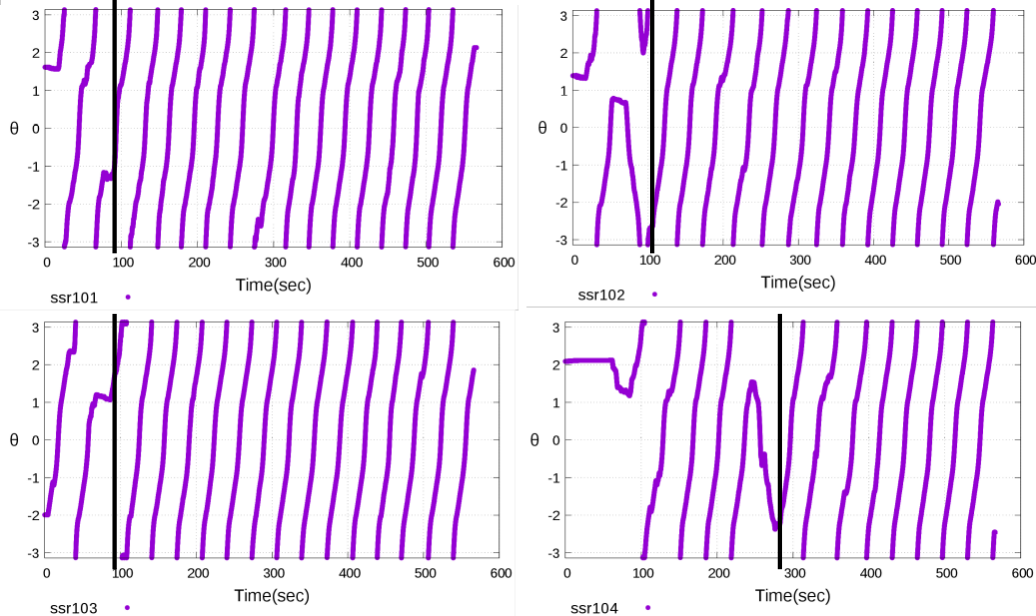
\includegraphics[width=1.0\linewidth]{ssr4_1.png}
\end{figure}

\vspace{-8mm}
\begin{figure}[!ht]\label{ssr2}
     \centering
     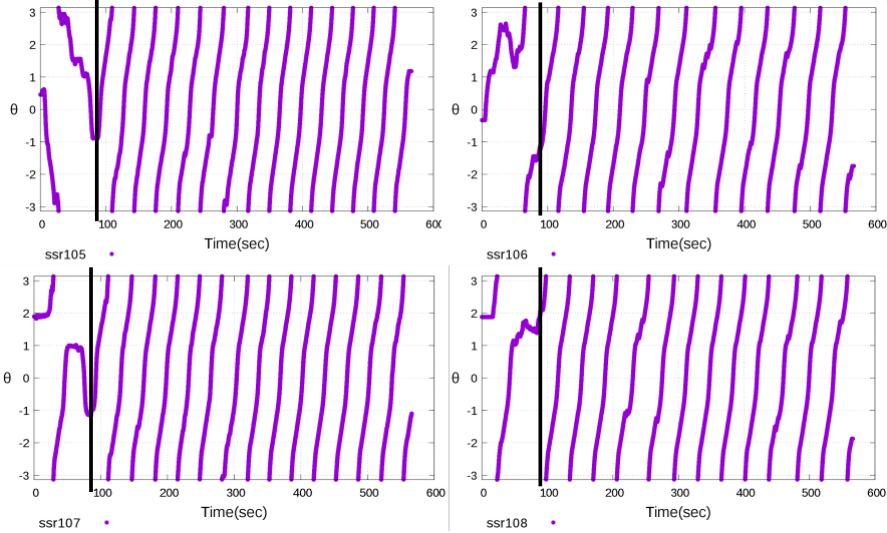
\includegraphics[width=1.0\linewidth]{ssr4_2.png}
     \caption{コース中心から見たロボットの角度$\theta$の時間変化}
     \label{fig:ssr}
\end{figure}


$T_{\rm 1d}$とは全てのロボットが方向転換せず,
同じ向きで走る(one direction flow)状態になる時間である,
図\ref{fig:ssr}中の黒い線はロボットが方向転換しなくなるまでの時間,
その中で一番長いものを$T_{\rm 1d}$とする.




